% Paper 1037, PacificVis 2027 Conference Paper Track. Source version v24 (2026-11-09; one-storm teaser, rewritten introduction, evaluation reordered), official VGTC conference template (vgtc.cls 2024/02/12).
% Build: pdflatex main && bibtex main && pdflatex main && pdflatex main   (or Overleaf / tectonic main.tex)
% Authors: edit \author{...} below (official VGTC conference format; single-blind, so no review option).
% Supplementary Material: supplement.tex (same folder, same figures/ and refs.bib).
\documentclass{vgtc}                % final conference style: authors shown (single-blind review)
%\documentclass[review]{vgtc}       % use only for double-blind review (hides authors, shows \onlineid)
\usepackage[T1]{fontenc}
\usepackage{mathptmx}
\usepackage{cite}
\usepackage{amsmath,amssymb,amsthm}
\usepackage{placeins}
\usepackage{booktabs,multirow,colortbl}
\makeatletter
\setlength{\@dblfptop}{0pt}
\setlength{\@dblfpsep}{12pt}
\setlength{\@dblfpbot}{0pt plus 1fil}
\makeatother
% Float placement only (no change to fonts or spacing): allow two full-width figures at the top of a page.
\setcounter{dbltopnumber}{2}
\usepackage[ruled,vlined]{algorithm2e}
\SetKwInput{KwData}{Data}
\SetKwInput{KwResult}{Result}
\SetKwProg{Fn}{Function}{:}{}
\SetKw{KwReturn}{return}
\SetKw{KwBreak}{break}
\SetKwFunction{Construct}{ConstructTemporalMap}
\SetKwFunction{Refine}{RefineOrder}
\SetKwFunction{Barriers}{OptimalBarriers}
\SetAlFnt{\small}
\SetAlCapFnt{\small\bfseries}
\SetAlCapNameFnt{\small\bfseries}
\SetAlCapSkip{3pt}
\DontPrintSemicolon
\setcounter{secnumdepth}{3}
\newtheorem{theorem}{Theorem}
\newtheorem{lemma}{Lemma}
\newtheorem{proposition}{Proposition}
\newcommand{\dtop}{d_{\mathrm{top}}}
\newcommand{\lca}{\operatorname{lca}}
\newcommand{\nroe}{\mathrm{NROE}}
\newcommand{\pos}[1]{\left[#1\right]^+}
% Only used for double-blind review (review option); harmless otherwise.
\onlineid{1037}
% Declare the category of your paper, only shown in review mode.
\vgtccategory{Research}
% Allow for this line if you want the electronic option to work properly.
\vgtcinsertpkg

% Paper title.
\title{AnchorMTM: Spatially Anchored Merge Tree Maps with Position Bounds}

\author{%
Lele~Wang$^{1,2}$\thanks{%
Affiliations:
$^{1}$ Advanced Interactive Technology and Application Laboratory, Computer Network Information Center, Chinese Academy of Sciences, Beijing, China;
$^{2}$ University of Chinese Academy of Sciences, Beijing, China;
$^{3}$ Hangzhou Institute for Advanced Study, UCAS, Hangzhou, China.
E-mails: lelewang@cnic.cn; dongyu@cnic.cn; yxmeng@cnic.cn;
liguan@sccas.cn; wangzhe@sccas.cn; shanghuihua@sccas.cn;
liujun@sccas.cn.
Lele Wang and Yu Dong contributed equally to this work.
Jun Liu is the corresponding author.}%
\quad
Yu~Dong$^{1,*}$%
\quad
Yuxiang~Meng$^{1,2}$%
\quad
Guan~Li$^{1,2}$%
\quad
Zhe~Wang$^{1,2}$%
\quad
Guihua~Shan$^{1,2,3}$%
\quad
Jun~Liu$^{1,2}$\thanks{Corresponding author. E-mail: liujun@sccas.cn.}
}

\hypersetup{pdftitle={AnchorMTM: Spatially Anchored Merge Tree Maps with Position Bounds},pdfauthor={Lele Wang, Yu Dong, Yuxiang Meng, Guan Li, Zhe Wang, Guihua Shan, Jun Liu}}
\teaser{
\centering
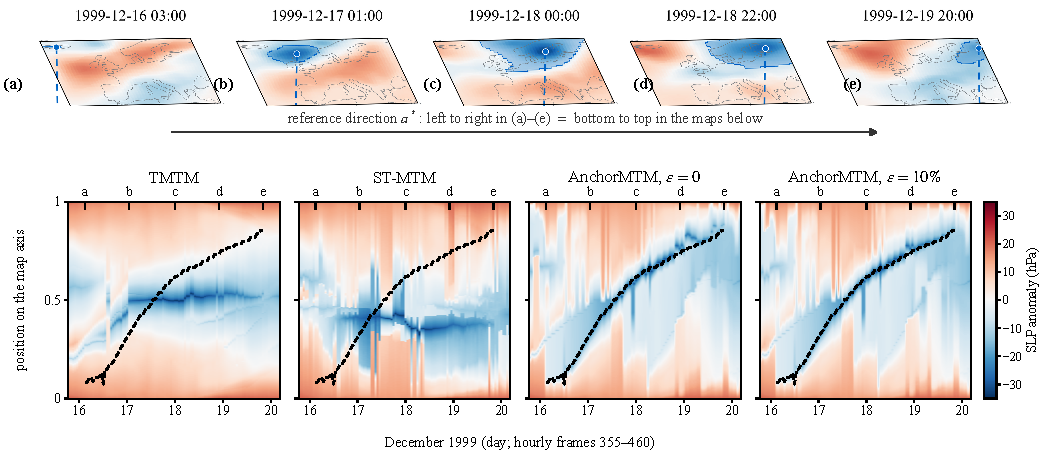
\includegraphics[width=\linewidth]{figures/teaser_storms_compare.pdf}
% Manual caption in the class format (\captionfonts, "Figure N:", justified): \caption inside \teaser
% prints an empty caption once \vgtcinsertpkg loads hyperref.
\par\vskip\abovecaptionskip
\refstepcounter{figure}\label{fig:storms_overview}%
{\captionfonts\leftskip=0pt\rightskip=0pt\parfillskip=0pt plus 1fil\noindent\figurename~\thefigure: One storm drawn by three merge tree maps. (a)--(e)~Sea-level-pressure anomaly over the North Atlantic and Europe between 16 and 19~December~1999; the marked minimum travels from the open Atlantic to Scandinavia. Below, TMTM, ST-MTM and AnchorMTM draw the same 106 hourly frames. The dashed line is the storm's location projected onto the reference direction, that is, where a map whose axis encodes location should draw it; ticks a--e mark the snapshot times. TMTM and ST-MTM keep the storm near the middle of the axis throughout. AnchorMTM follows it with exact topology ($\varepsilon=0$; mean deviation 1.5\% of the axis) and with a 10\% merge budget (1.0\%). Hourly Storms archive, prepared separately from Table~\ref{tab:quantitative-final}.\par}
}

\abstract{Merge tree maps summarize a time-varying scalar field in one static image. Each time step becomes a one-dimensional profile of its merge tree, and the profiles are stacked along time, so that nested features appear as nested bands. Existing maps arrange the profiles to keep the hierarchy intact and the bands temporally coherent. The vertical position of a band therefore has no fixed spatial meaning, and an analyst cannot read where a feature is or in which direction it moves. We anchor this axis to a spatial direction and draw every feature near the projection of its location. Anchoring conflicts with the merge tree: an exact profile places each subtree in one contiguous block, whereas the projected locations of sibling subtrees may interleave. We show that the displacement caused by this conflict can be computed. We formulate merge tree maps, including TMTM and ST-MTM, as instances of one layout problem and derive three lower bounds on the displacement that every instance must accept under exact topology, finite feature widths and a bounded change of merge levels. The bounds require no layout, so they separate the error that a tree forces from the error that a layout chooses. AnchorMTM approaches the bounds and exposes a single parameter, a merge-error budget. The bounds are attained on 606 of 614 benchmark frames, and 31--95\% of the order error of TMTM and ST-MTM is not forced by the tree. At zero merge error, AnchorMTM reduces the mean worst displacement by 73--96\% on the four planar inputs of the ST-MTM benchmark and an hourly PM$_{2.5}$ sequence and by 63--67\% on two volumes, while ST-MTM retains better neighborhood preservation.}
\keywords{Time-varying scalar fields, merge tree maps, topology preservation, spatial fidelity, lower bounds, constrained layout.}
\begin{document}
\firstsection{Introduction}
\maketitle
\raggedbottom
\setlength{\emergencystretch}{1.5em}
Time-varying scalar fields record how quantities such as sea-level pressure, aerosol concentration or vorticity evolve over a spatial domain. Analysts study them through features, such as low-pressure systems, pollution episodes or vortices, and ask three kinds of questions: which features exist and how they relate, where they are, and how they move. Animation shows each time step in its spatial context but makes distant times hard to compare~\cite{Tversky:2002:Animation,Robertson:2008:Animation}. Static overviews instead assign one display axis to time and compress the spatial domain into the other, so that a whole sequence can be compared at a glance~\cite{Bach:2017:STC}. In atmospheric science, the Hovm\"oller diagram is the standard example: its second axis is a physical coordinate such as longitude, and the eastward drift of a weather system appears as a slanted streak~\cite{Hovmoller:1949}.

Topology offers a more structured overview. A merge tree records how the sublevel sets of a field connect as the threshold rises; its leaves are the extrema, and its internal nodes are the levels at which regions merge~\cite{Heine:2016:Survey}. Temporal merge tree maps (TMTM) draw the merge tree of every time step as a one-dimensional profile, whose minima are the extrema and whose barriers are the merge levels, and stack the profiles into one image~\cite{Koepp:2023:TMTM}. Spatiotemporal merge tree maps (ST-MTM) additionally place features according to their pairwise distances~\cite{STMTM:2026}. Both make the nesting and the merge thresholds of all features visible in a single image, which neither animation nor a Hovm\"oller diagram provides.

These maps, however, lack a spatial axis. TMTM orders features by the tree and by temporal alignment, and ST-MTM preserves relative distances, which fix neither an origin nor a direction. Figure~\ref{fig:storms_overview} shows the consequence for one storm. Between 16 and 19~December~1999, the storm travels from the open Atlantic to Scandinavia, yet both maps draw its band near the middle of the axis for the entire period. A reader can follow the storm and its connections to neighboring lows, but not its position or the direction of its motion. A Hovm\"oller diagram would show the motion, but it averages away the hierarchy that motivates a merge tree map in the first place.

Giving a merge tree map a spatial axis is harder than it appears. Projecting each extremum onto a reference direction yields a target position, but the merge tree restricts which positions are admissible: a profile that shows the tree exactly must keep every subtree in one contiguous block. When the projected locations of two sibling subtrees interleave, as in Figure~\ref{fig:projection_conflict}, no exact profile can place all features at their targets. This conflict is a property of the data rather than of a particular layout algorithm, and it raises three questions that existing work leaves open: how much displacement the tree forces, where in the tree the displacement originates, and how much merge-level fidelity must be given up to remove it. Without answers, one cannot tell whether the positional error of a map is inherent or a weakness of its layout, nor decide whether a spatial axis is worth its cost.

We address these questions in three steps. We first express existing merge tree maps as instances of one layout problem, which makes their axes and their errors comparable. We then derive lower bounds on the displacement that every instance must accept, for exact topology, for features of finite width and for a bounded change of merge levels. The bounds depend only on the tree, the projected locations and the widths; they can be computed before any map is drawn and applied to any existing map. Finally, we present AnchorMTM, a construction of spatially anchored merge tree maps that approaches these bounds. A single parameter, the merge-error budget $\varepsilon$, determines how much merge-level fidelity may be traded for position. With $\varepsilon=0$, the map keeps the tree exactly; with $\varepsilon>0$, every frame reports the merge error it actually spends.

In summary, we contribute
\begin{itemize}
\setlength{\itemsep}{2pt}
\setlength{\parsep}{0pt}
\item a formulation of merge tree maps as one constrained layout problem, with TMTM and ST-MTM as exact-topology instances, and three layout-independent lower bounds on the displacement caused by the conflict between position and topology (Sections~\ref{sec:formulation} and~\ref{sec:bounds});
\item AnchorMTM, a spatially anchored merge tree map that approaches these bounds and controls the trade-off with a single merge-error budget (Section~\ref{sec:method});
\item an evaluation on five planar and two volumetric sequences showing that the bounds are tight, that most of the positional error of existing maps is avoidable, and how a budget changes the map (Section~\ref{sec:experiments}).
\end{itemize}

\section{Related Work}\label{sec:related}
\subsection{Temporal Overviews of Spatial Data}
Animation preserves the spatial context of each time step, whereas static overviews let viewers compare distant times directly; which one serves better depends on the task~\cite{Tversky:2002:Animation,Robertson:2008:Animation}. Bach et al.\ describe both, and the operations between them, as transformations of a space--time cube~\cite{Bach:2017:STC}. A static overview has to linearize space. Hovm\"oller diagrams keep one physical coordinate and average over the others~\cite{Hovmoller:1949}. Geographic orderings, dense pixel displays and space-filling curves traverse the whole domain~\cite{Guo:2006:SpatialOrder,Dafner:2000:CSFC,Rauscher:2025:1DO}, and volume lines and data-driven curves extend such traversals to volumes~\cite{Weissenboeck:2019:DVL,Zhou:2021:DSF}. For moving objects, one-dimensional projections and summaries such as MotionRugs, stable visual summaries and MoReVis order objects by position or by stability~\cite{Franke:2021:1DP,Buchmueller:2019:MR,Wulms:2021:SVS,Valdrighi:2024:MRV}. Each of these linearizations distorts some spatial relations~\cite{Nonato:2019:MP,Aupetit:2007:VD}. They keep a spatial coordinate but no feature hierarchy; our maps keep the merge tree and quantify what the spatial coordinate then costs.

\subsection{Topology of Time-Varying Scalar Fields}
Merge trees and contour trees summarize how level sets connect, and persistence-based simplification controls their size~\cite{Heine:2016:Survey,Edelsbrunner:2002:TPS,Tierny:2018:TTK}. Features are tracked over time by region overlap or attribute similarity~\cite{Silver:1997:Tracking,Saikia:2017:GFT} and shown as tracking graphs and nested tracking graphs~\cite{Widanagamaachchi:2012:DTG,Lukasczyk:2017:NTG,Lukasczyk:2020:DNTG}. Time-varying merge trees have been computed and compared with Wasserstein and geometry-aware interleaving distances~\cite{Oesterling:2017:TVMT,Pont:2022:WMT,Yan:2022:GAMT,Yan:2021:Survey}, and such pipelines have been used to follow tropical cyclones and atmospheric rivers~\cite{Yan:2024:TROPHY,Lan:2024:AR}. The merge error we bound is a labelled interleaving distance~\cite{Munch:2019:LINF,Gasparovic:2024:IID,Morozov:2013:IDMT} and is related to distances between ordered merge trees~\cite{Beurskens:2025:OMT}. Tracking graphs show how features appear, split and merge, but not where they are; merge tree maps also show the values and the nesting of every time step.

\subsection{Drawing Hierarchies in One Dimension}
Topological landscapes draw a merge tree as a terrain or as a one-dimensional profile whose minima are the extrema and whose barriers are the merge levels~\cite{Weber:2007:TL,Oesterling:2013:TLP}; geometry-preserving and temporally coherent variants exist~\cite{Beketayev:2012:GPTL,Herick:2020:TCTL}, and contour trees have also been drawn in the plane and in joint layouts~\cite{Heine:2011:DCT,Lohfink:2020:FCT}. Temporal treemaps lay out evolving hierarchies along time~\cite{Koepp:2019:TT}. TMTM aligns the profiles of successive merge trees into one static map~\cite{Koepp:2023:TMTM}, and ST-MTM adds relative spatial distances and temporal stability~\cite{STMTM:2026}. Storyline layouts face a related problem for groups of entities and balance crossings and wiggles against group contiguity~\cite{Tanahashi:2012:Storyline,Liu:2013:SF}. To our knowledge, TMTM and ST-MTM are the only methods that produce the output we study, a static map of merge tree profiles over time, and they are therefore our direct baselines. Table~\ref{tab:family} relates them to tree-only orderings and space-only linearizations, and Section~\ref{sec:experiments} measures all of them.

\subsection{Hierarchies against an External Order}
The conflict we study arises whenever a tree must respect an external order. Optimal leaf ordering selects a tree-consistent order of a dendrogram that keeps similar leaves adjacent~\cite{BarJoseph:2001:OLO,Eisen:1998:CA}, and tree reordering seeks the tree-consistent permutation closest to a target order~\cite{Bulteau:2022:RT}. Spatially ordered treemaps and data--spatial grid maps trade hierarchy or data layout against geographic position~\cite{Wood:2008:SOT,vanBeusekom:2023:DSL}, geophylogenies connect leaf orders to map locations~\cite{Klawitter:2025:GP}, and tanglegram layouts minimize crossings or displacement between two trees~\cite{Fernau:2010:CTC,Huson:2026:DOT}. Separation constraints keep laid-out objects disjoint~\cite{Dwyer:2006:IPSEP,Li:2019:SOI}, ultrametric fitting under the maximum norm is closely related to our optimal barriers~\cite{Farach:1995:RM}, and merge distortion and topology-preserving projections measure how much hierarchy a mapping retains~\cite{Eldridge:2015:MD,Doraiswamy:2021:TM}. These methods optimize crossings, sums or stress for a given instance. We instead bound, in closed form for points, the worst displacement that every tree-consistent layout must accept, together with the merge error that removes it.

\section{Spatially Anchored Merge Tree Maps}\label{sec:formulation}
We first describe merge tree maps by one formulation that covers the existing ones, then give the axis a spatial reference and show where it conflicts with the tree.

\subsection{Merge Trees and One-Dimensional Profiles}\label{sec:background}
For a scalar field $f_t$ on a 2D or 3D domain, the merge tree $T_t$ records how sublevel-set components appear at minima and join at saddles as the threshold increases; negating the field gives the split tree~\cite{Heine:2016:Survey,Tierny:2018:TTK}. Persistence simplification precedes layout, and all statements refer to the simplified tree~\cite{Edelsbrunner:2002:TPS}. Each leaf $i$ is an extremum at location $p_i^t$; its support $S_i^t$ is the set of samples on its leaf arc, with measure $m_i^t$. Two leaves merge at the level $V_{ij}^t=h_t(\lca(i,j))$ of their lowest common ancestor, and $V_{ii}^t$ is the extremum value; equal-level merges form one multifurcation.

A one-dimensional profile draws the leaves as minima in a chosen leaf order, each inside an interval sized by its support, and fills the gaps from the tree, so that the largest profile value between two minima shows their merge level~\cite{Weber:2007:TL,Oesterling:2013:TLP,Koepp:2023:TMTM}. The profile shows the tree exactly only if every subtree occupies one contiguous block of leaves. Stacking the profiles along time gives a temporal merge tree map; leaves of consecutive frames are matched by support overlap with a one-to-one assignment, and $\mu_t(i)$ denotes the matched predecessor of leaf $i$~\cite{STMTM:2026}.

\subsection{A Common Formulation}\label{sec:common}
A map frame consists of a leaf order $\pi$, intervals with centers $z_i$ and widths $W_i$, display anchors $x_i$ for the extrema, and a profile $\psi$. The layout set $\mathcal{L}(\pi;W)$ contains the placements whose intervals follow $\pi$ on the canvas $[0,L]$, are disjoint with gap at least $g$, and hold each anchor within $\rho W_i/2$ of its center. Two errors describe a frame. The \emph{merge error} compares displayed and true merge levels of fixed labels,
\begin{equation}\label{eq:dtop}
 \dtop(\psi,T)=\max_{i,j}\bigl|V_{ij}^{\psi}-V_{ij}\bigr|,
\end{equation}
where $V_{ij}^{\psi}$ is the largest profile value between the anchors of $i$ and $j$. It is zero exactly when the profile shows the tree, and for complete labels it equals the labelled interleaving distance, which bounds the interleaving and bottleneck distances~\cite{Munch:2019:LINF,Gasparovic:2024:IID,Morozov:2013:IDMT}. The \emph{positional error} compares anchors with spatial targets $q_i$ (Section~\ref{sec:reference}); its worst value $\|x-q\|_\infty$ is reported per frame. Two order-level versions isolate the role of the leaf order:
\begin{equation}\label{eq:nroe}
\begin{aligned}
 \nroe(\pi)&=\frac{1}{2L}\max_{j\le k}\bigl[q_{\pi(j)}-q_{\pi(k)}\bigr]^+,\\
 \tau(\pi)&=\min_{(x,z)\in\mathcal{L}(\pi;W)}\|x-q\|_\infty .
\end{aligned}
\end{equation}
NROE is the smallest worst displacement of points placed in order $\pi$, relative to $L$; $\tau$ adds the intervals and is computed exactly for a fixed order.

Each map we consider solves, frame by frame, an instance of
\begin{equation}\label{eq:family}
\begin{aligned}
 \min_{\pi\in\Pi,\;(x,z)\in\mathcal{L}(\pi;W)}\;&\lambda_R E_R+\lambda_G E_G+\lambda_M E_M+\lambda_C E_C\\
 \mathrm{s.t.}\;&\dtop(\psi,T)\le\eta .
\end{aligned}
\end{equation}
Here $E_R$ is the mean squared distance of anchors to their references, $E_G$ a stress between anchor separations and support-centroid distances, $E_M$ the mean squared distance to a temporal target $\hat x_i$ derived from the matched previous anchor, and $E_C$ the offset of anchors from interval centers. A method is a choice of order rule $\Pi$, weights $\lambda$, temporal target $\hat x$, width semantics $W$ and allowance $\eta$ (Table~\ref{tab:family}). TMTM and ST-MTM keep the tree ($\eta=0$) and have no reference term ($\lambda_R=0$): TMTM greedily orders children by subtree overlap between frames and packs intervals by sample count~\cite{Koepp:2023:TMTM}, whereas ST-MTM picks a temporally concordant or optimal leaf order within the tree and fits relative distances~\cite{STMTM:2026}. Their axes therefore encode tree traversal or relative distance rather than location. Projections and space-filling curves sit at the other end: they follow space and ignore the tree~\cite{Franke:2021:1DP}. AnchorMTM adds the reference term and a declared allowance $\eta$, controlled by one number $\varepsilon$ (Section~\ref{sec:method}). The correspondence concerns the problem each method solves. Solvers differ in scaling and other details, and Section~\ref{sec:experiments} evaluates implementations of the published methods, not our solver with their weights.

\begin{table}[t]
\centering
\caption{Maps of time-varying scalar fields as instances of Eq.~\ref{eq:family}. Order rule: how leaves are ordered; placement: nonzero terms and temporal target; $\eta$: allowed merge error relative to the scalar range (tolerance $\varepsilon_0$ omitted); axis: what a position encodes.}
\label{tab:family}
\footnotesize
\setlength{\tabcolsep}{2pt}
\renewcommand{\arraystretch}{1.05}
\begin{tabular*}{\columnwidth}{@{\extracolsep{\fill}}>{\raggedright\arraybackslash}p{0.19\columnwidth}>{\raggedright\arraybackslash}p{0.25\columnwidth}>{\raggedright\arraybackslash}p{0.25\columnwidth}c>{\raggedright\arraybackslash}p{0.13\columnwidth}@{}}
\toprule
Method & Order rule & Placement & $\eta$ & Axis \\
\midrule
TMTM~\cite{Koepp:2023:TMTM} & greedy child order by subtree overlap between frames & packed by sample count; no anchor optimization & 0 & tree traversal \\
ST-MTM~\cite{STMTM:2026} & concordant order unless OLO is cheaper by a ratio & $\lambda_G$ (stress), $\lambda_M$ on matched anchors, then intervals & 0 & relative distance \\
OLO~\cite{BarJoseph:2001:OLO} & tree-constrained OLO & ranks only & 0 & order \\
Projection, Hilbert, Morton~\cite{Franke:2021:1DP} & by reference or curve & at reference or curve rank & none & location or curve rank \\
\midrule
AnchorMTM & least $\tau$ within the budget & $\lambda_R$ dominant, $\hat x$ follows projected motion & $\varepsilon$ & location \\
\bottomrule
\end{tabular*}
\end{table}


\subsection{Spatial Reference}\label{sec:reference}
A reference gives the axis a meaning: $q_i^t=\langle a,p_i^t\rangle-o$ for one unit direction $a$ and one origin $o$, where $o$ and the extent $L$ come from the projected corners of the domain. By default, $a$ is the direction of largest matched extremum motion,
\begin{equation}\label{eq:autodirection}
 a^*\in\arg\max_{\|a\|=1}\;a^\top\Bigl(\sum_{t,i}\Delta p_i^t(\Delta p_i^t)^\top\Bigr)a,
\end{equation}
with $\Delta p_i^t=p_i^t-p_{\mu_t(i)}^{t-1}$
over valid matches, signed so that the total projected motion is nonnegative; a direction chosen by the analyst can replace it. Direction, origin and extent are fixed for the whole sequence and all budgets, without per-frame recentering, so a feature that moves along $a$ moves along the axis. Matching by support overlap can miss fast features, which then contribute no motion sample.

\subsection{Where Topology and Space Conflict}\label{sec:conflict}
\begin{figure}[t]
\centering
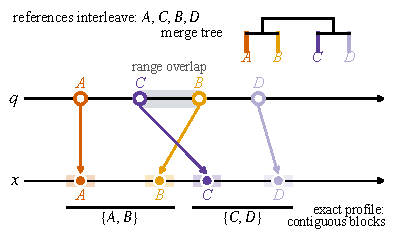
\includegraphics[width=\columnwidth]{figures/anchor_conflict_v23.pdf}
\caption{Reference--topology conflict. The merge tree requires the blocks $\{A,B\}$ and $\{C,D\}$, but the references occur in the order $A,C,B,D$. Every exact profile must therefore move some anchors away from their references (arrows). The overlap of the two subtrees' reference ranges (grey) determines the least displacement (Theorem~\ref{thm:order}). Positions are schematic.}
\label{fig:projection_conflict}
\end{figure}
An exact profile keeps every subtree contiguous, but the references of sibling subtrees may interleave. In Fig.~\ref{fig:projection_conflict} the references occur in the order $A,C,B,D$: $C$ lies between $A$ and $B$, and $B$ between $C$ and $D$. Neither arrangement of the blocks $\{A,B\}$ and $\{C,D\}$ matches this order, so no exact profile places all four anchors at their references, and finite widths add packing constraints. Section~\ref{sec:bounds} determines how large the displacement must be, where it arises and how much merge error removes it. The answer depends only on $T$, $q$, $W$ and $\eta$, and therefore holds for every instance of Eq.~\ref{eq:family} at once.

\section{The Positional Price of Keeping the Tree}\label{sec:bounds}
The three bounds below involve the tree, the references, the widths and the allowance, but neither the order rule nor the weights, so they hold for every row of Table~\ref{tab:family}. The first concerns exact topology, the second adds widths, and the third allows a merge error. Full proofs are in the Supplementary Material; within a frame we drop $t$, write $[v]^+=\max(v,0)$, and take empty maxima as zero.

\subsection{Exact Topology}
On the reduced tree, where equal-level merges form one node, exact topology makes every subtree contiguous. Let $[m_X,M_X]$ be the reference range of the leaves of subtree $X$.
\begin{theorem}[Exact-Topology Position Bound]\label{thm:order}
Every profile with $\dtop=0$ has $\nroe(\pi)\ge\nu^*(T,q)$, where
\begin{equation}\label{eq:nu}
 \nu^*(T,q)=\frac{1}{2L}\max_v\max_{\substack{X,Y\in\mathrm{ch}(v)\\X\ne Y}}
 \bigl[\min(M_X-m_Y,\,M_Y-m_X)\bigr]^+ .
\end{equation}
Ordering children recursively by the midpoints of their reference ranges attains $\nu^*$ in $O(n\log n)$ time.
\end{theorem}
\begin{proof}[Proof sketch]
Two sibling blocks must take one of two orientations, with inversion costs $[M_X-m_Y]^+/2$ and $[M_Y-m_X]^+/2$; midpoint order takes the smaller, and every inverted pair of leaves is separated by sibling blocks at its lowest common ancestor.
\end{proof}
The maximizing node and sibling pair locate the price at the merge of two subtrees whose reference ranges overlap, and its value is half the overlap left in the cheaper orientation. In Fig.~\ref{fig:projection_conflict} the ranges of $\{A,B\}$ and $\{C,D\}$ overlap by $q_B-q_C$, so every exact profile has an order error of at least $(q_B-q_C)/2L$.

\paragraph{Forced and chosen error.} Because midpoint ordering attains $\nu^*$ on the same tree, the order error of any exact-topology map splits into $\nu^*(T,q)$, which the tree forces, and $\nroe(\pi)-\nu^*(T,q)$, which its order rule chooses and which can be removed without changing the tree. NROE does not involve widths, so the split applies equally to TMTM and ST-MTM, whose interval sizes follow different rules.

\subsection{Finite Widths}
Intervals need room: a block of leaves occupies at least the sum of its widths and gaps. For disjoint leaf sets $X$ and $Y$, let $\omega(X,Y)$ be the least worst displacement that placing all of $X$ before all of $Y$, or the reverse, whichever is smaller, forces on their anchors, and let $E_\partial$ be the cost of fitting all intervals between the canvas ends. Both follow from sorted reference endpoints and cumulative widths (Supplementary Material).
\begin{theorem}[Width-Aware Position Bound]\label{thm:width}
Let $\mathcal{P}_0$ contain every pair of descendant-leaf sets of two siblings. Every exact-topology interval layout satisfies
\begin{equation}\label{eq:widthbound}
\begin{aligned}
 \|x-q\|_\infty\ge\tau(\pi)&\ge\mathcal{B}_w(T,q,W)\\
 &=\max\Bigl\{E_\partial,\max_{(X,Y)\in\mathcal{P}_0}\omega(X,Y)\Bigr\}.
\end{aligned}
\end{equation}
With zero widths and gaps, $\mathcal{B}_w=L\,\nu^*(T,q)$.
\end{theorem}
\begin{proof}[Proof sketch]
The first and last anchors of a block must enclose its intervals and gaps up to the anchor slack, which gives a shortfall against the reference separation; exact topology fixes one orientation of every sibling pair, and the canvas ends give the one-sided costs.
\end{proof}
$\mathcal{B}_w$ bounds every exact-topology order and need not be attained; $\tau(\pi)$ is the attained minimum for a given order.

\subsection{A Bounded Merge Error}
A merge allowance can release a block, but it still limits interleaving. If leaf $k$ lies between two descendants $i,j$ of node $u$, its displayed merge with $i$ cannot exceed theirs, so $V_{ik}\le h(u)+2\eta$. Leaf $k$ can therefore enter the block of $u$ only if it descends from $A_\eta(u)$, the highest ancestor of $u$ whose level is within $2\eta$ of $h(u)$. Let $\mathcal{P}_\eta$ contain the leaf-set pairs that this rule keeps apart: $(\mathcal{D}(u),\{k\})$ for leaves $k$ outside $\mathcal{D}(A_\eta(u))$, and $(\mathcal{D}(u),\mathcal{D}(w))$ for internal nodes $u,w$ with $\mathcal{D}(w)$ disjoint from $\mathcal{D}(A_\eta(u))$ and $\mathcal{D}(u)$ disjoint from $\mathcal{D}(A_\eta(w))$, where $\mathcal{D}(\cdot)$ denotes descendant leaves.
\begin{theorem}[Bounded-Topology Position Bound]\label{thm:chain}
In every profile with $\dtop\le\eta$, each pair in $\mathcal{P}_\eta$ lies wholly in one orientation. Hence
\begin{equation}\label{eq:chainbounds}
\begin{aligned}
 \nroe(\pi)&\ge C_\eta=\max_{(X,Y)\in\mathcal{P}_\eta}\frac{[\min(M_X-m_Y,M_Y-m_X)]^+}{2L},\\
 \tau(\pi)&\ge\max\Bigl\{E_\partial,\max_{(X,Y)\in\mathcal{P}_\eta}\omega(X,Y)\Bigr\}.
\end{aligned}
\end{equation}
\end{theorem}
The theorem also states what releases a conflict. A subtree may interleave with its sibling once $2\eta$ reaches the gap between its own merge level and that of its parent, so conflicts at deep merges remain expensive. Flattening every parent gap of at most $2\eta$ gives a second valid bound; neither dominates the other, and we report the larger. Read in reverse, the theorem also prices the other end of Table~\ref{tab:family}: a map whose order error is below $C_\eta$, such as a projection with zero order error, must show a merge error above $\eta$.

\section{AnchorMTM: Approaching the Bounds}\label{sec:method}
\begin{figure*}[t]
\centering
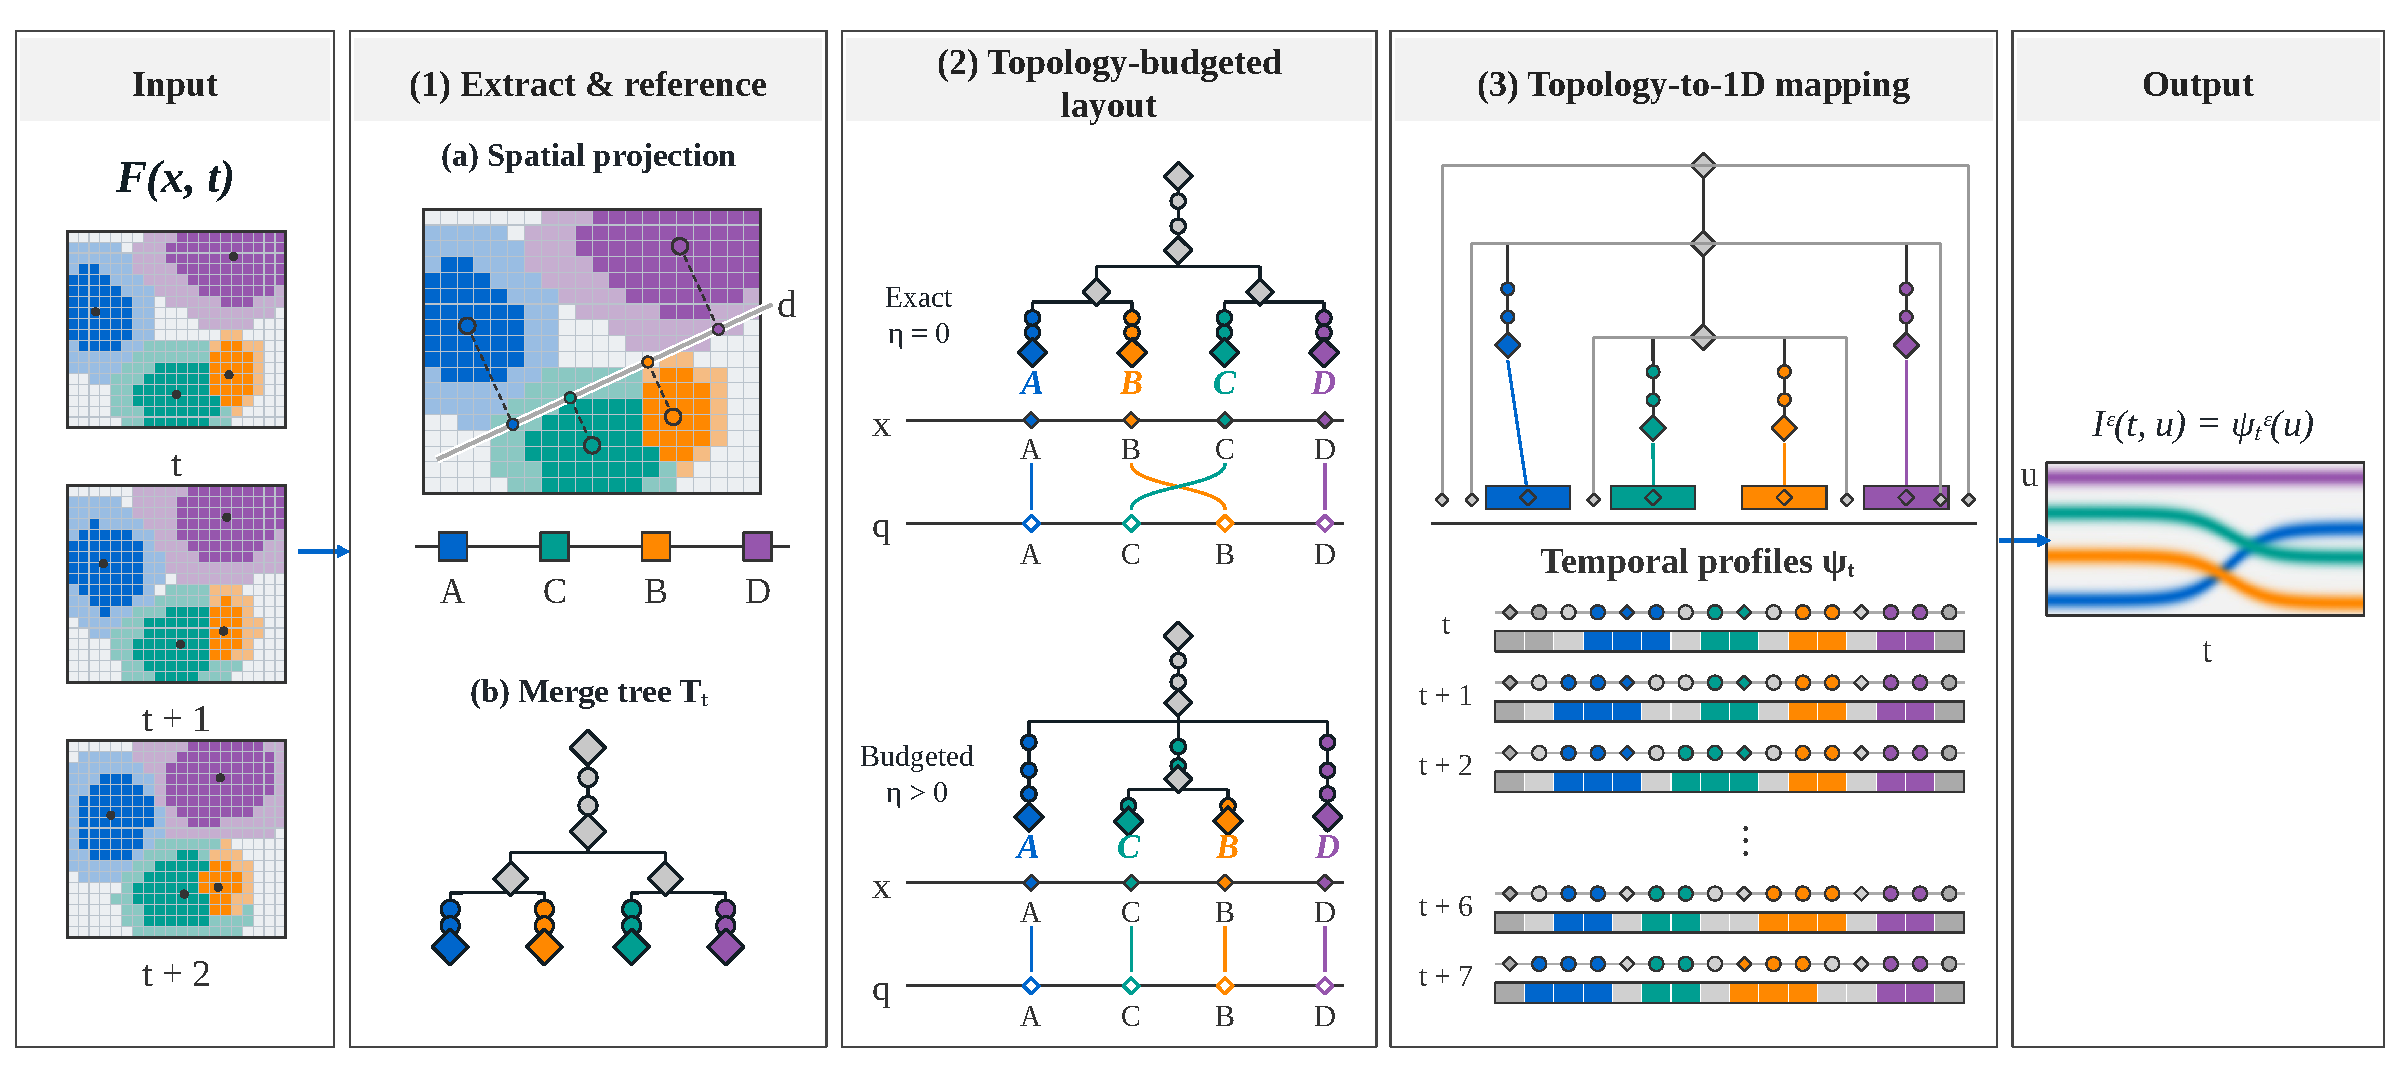
\includegraphics[width=\textwidth]{figures/anchor_framework.pdf}
\caption{AnchorMTM construction (schematic; $F(x,t)$ denotes the field at location $x$ and time $t$). (1) Extract and reference: merge trees of each frame, leaf supports matched across frames, and one fixed direction $d$ (the $a^*$ of Eq.~\ref{eq:autodirection}) that gives every extremum its reference position $q$. (2) Topology-budgeted layout: search leaf orders admitted by the budget $\eta$, then place anchors $x$ under a displacement cap; with $\eta=0$ the order keeps the subtree blocks and anchors leave their references, whereas $\eta>0$ admits an order that follows them. (3) Topology-to-1D mapping: fill intervals and barriers into each profile $\psi_t$ and stack the profiles over time into the map $I^\varepsilon(t,u)=\psi^\varepsilon_t(u)$.}
\label{fig:framework}
\end{figure*}
AnchorMTM is the instance of Eq.~\ref{eq:family} with a reference term and the allowance $\eta=(\varepsilon_0+\varepsilon)\Delta_F$, where $\Delta_F$ is the scalar range of the sequence, $\varepsilon_0=10^{-7}$ a fixed numerical tolerance, and $\varepsilon\ge0$ the only control. \emph{Exact Mode} ($\varepsilon=0$) keeps the tree up to ties within $\varepsilon_0\Delta_F$; \emph{Budgeted Mode} ($\varepsilon>0$) trades a declared merge error for position. Because Eq.~\ref{eq:family} couples a discrete order with continuous placement, AnchorMTM solves it in two stages that follow the bounds (Fig.~\ref{fig:framework}, panel~2): it chooses the order by $\tau$, the quantity that the bounds constrain, and then places anchors within a cap on $\tau$. Intervals have widths $W_i=s\,m_i$ with one fixed scale $s$; all other settings form one fixed configuration, listed in the Supplementary Material.

\subsection{Leaf Order within the Budget}
For each frame, the order is chosen lexicographically,
\begin{equation}\label{eq:orderobjective}
 \pi^\varepsilon\in\underset{\pi\in\mathcal{C}}{\arg\min}\bigl(\tau(\pi),\nroe(\pi)\bigr)
 \quad\mathrm{s.t.}\quad\delta^*(\pi)\le\eta ,
\end{equation}
over a finite candidate pool $\mathcal{C}$: the exact tree ordered by midpoints, which attains $\nu^*$, threshold and conflict-driven flattenings of the tree, and the orders visited while width-aware block moves refine the best of them. Every candidate is evaluated against the original merge matrix. The pool is heuristic, so the selected order is not a certified optimum over all permutations; Section~\ref{sec:experiments} measures how often it attains the bounds. Admission uses the smallest merge error that an order can show.
\begin{proposition}[Optimal Barriers]\label{prop:barriers}
For a fixed order, let $C_k=\min_{i\le k<j}V_{\pi(i)\pi(j)}$ be the lowest merge across gap $k$ and $F_k$ the larger of its two adjacent extremum values. The smallest attainable merge error is
\begin{equation}\label{eq:delta}
\begin{split}
 \delta^*(\pi)=\max\Bigl\{&0,\;\max_k(F_k-C_k),\\
 &\tfrac12\max_{i<j}\bigl(V_{\pi(i)\pi(j)}-\max_{i\le k<j}C_k\bigr)\Bigr\},
\end{split}
\end{equation}
attained by the barriers $b_k=C_k+\delta^*(\pi)$.
\end{proposition}
An order therefore meets the budget exactly when $\delta^*(\pi)\le\eta$, and admission becomes a closed-form test.

\subsection{Anchor Placement}
For the selected order, AnchorMTM solves Eq.~\ref{eq:family} with default weights $(\lambda_R,\lambda_G,\lambda_M,\lambda_C)=(4,1,0.5,0.1)$, the temporal target $\hat x_i^t=x_{\mu_t(i)}^{t-1}+(q_i^t-q_{\mu_t(i)}^{t-1})$, which follows projected motion and keeps $x-q$ continuous, and the additional cap $\|x-q\|_\infty\le\tau(\pi)+\beta_0$ with a fixed slack $\beta_0$. The cap is feasible because $\tau$ is attained, and for a fixed order the problem is a convex quadratic program. The program cannot replace the selected order, so the cap transfers the positional guarantee of the order to the anchors. Leaves without a matched predecessor have no temporal term.

\subsection{Profile Reconstruction and Checks}
Profiles reuse the leaf-arc sampling and the filling along paths to the lowest common ancestor of merge tree maps~\cite{Koepp:2023:TMTM,STMTM:2026}; extrema stay at their anchors, and each gap is then clipped or raised to its barrier $b_k$, as relaxed orders require. All frames share the direction, origin, extent and pixel scale, without per-frame recentering. Raster rounding and strict-extremum clearance can change the displayed merge levels, so every rendered frame is checked against the original merge matrix, and the records keep the requested budget, $\tau$, $\delta^*$ and the measured errors. Capacity, input and solver failures are reported rather than repaired by rescaling.

\section{Evaluation}\label{sec:experiments}
\definecolor{pubgray}{gray}{0.45}
\begin{table*}[t]
\centering
\caption{Five-dataset comparison. Bold/underline mark the best/second distinct local measurements per dataset; ties share emphasis. Curves use fixed default orientations.}
\label{tab:quantitative-final}
\footnotesize
\setlength{\tabcolsep}{1.5pt}
\renewcommand{\arraystretch}{0.85}
\begin{tabular*}{\textwidth}{@{\extracolsep{\fill}}l*{12}{c}lccc@{}}
\toprule
\multirow{2}{*}{Dataset} & \multicolumn{3}{c}{Hilbert} & \multicolumn{3}{c}{Morton} & \multicolumn{3}{c}{TMTM} & \multicolumn{3}{c}{ST-MTM} & \multicolumn{4}{c}{AnchorMTM (ours)} \\
\cmidrule(lr){2-4}\cmidrule(lr){5-7}\cmidrule(lr){8-10}\cmidrule(lr){11-13}\cmidrule(lr){14-17}
 & SNS$\downarrow$ & TW$\uparrow$ & NPE$\downarrow$ & SNS$\downarrow$ & TW$\uparrow$ & NPE$\downarrow$ & SNS$\downarrow$ & TW$\uparrow$ & NPE$\downarrow$ & SNS$\downarrow$ & TW$\uparrow$ & NPE$\downarrow$ & Mode & SNS$\downarrow$ & TW$\uparrow$ & NPE$\downarrow$ \\
\midrule
\multirow{2}{*}{Gaussian} & \multirow{2}{*}{$0.1117$} & \multirow{2}{*}{$0.6719$} & \multirow{2}{*}{$0.7557$} & \multirow{2}{*}{$\underline{0.0393}$} & \multirow{2}{*}{$\underline{0.8333}$} & \multirow{2}{*}{$0.7359$} & \multirow{2}{*}{\textcolor{pubgray}{$0.2500^\dagger$}} & \multirow{2}{*}{\textcolor{pubgray}{$0.7700^\dagger$}} & \multirow{2}{*}{$\underline{0.1118}$} & \multirow{2}{*}{\textcolor{pubgray}{$0.0600^\dagger$}} & \multirow{2}{*}{\textcolor{pubgray}{$1.0000^\dagger$}} & \multirow{2}{*}{$0.1154$} & Exact & $\mathbf{0.0353}$ & $\mathbf{0.9323}$ & $\mathbf{0.0089}$ \\
 &  &  &  &  &  &  &  &  &  &  &  &  & Balanced & $\mathbf{0.0353}$ & $\mathbf{0.9323}$ & $\mathbf{0.0089}$ \\
\multirow{2}{*}{Ring} & \multirow{2}{*}{$\mathbf{0.1252}$} & \multirow{2}{*}{$\mathbf{0.9048}$} & \multirow{2}{*}{$0.5941$} & \multirow{2}{*}{$0.1489$} & \multirow{2}{*}{$0.7619$} & \multirow{2}{*}{$0.6033$} & \multirow{2}{*}{\textcolor{pubgray}{$0.2800^\dagger$}} & \multirow{2}{*}{\textcolor{pubgray}{$0.6800^\dagger$}} & \multirow{2}{*}{$0.1756$} & \multirow{2}{*}{\textcolor{pubgray}{$0.2100^\dagger$}} & \multirow{2}{*}{\textcolor{pubgray}{$0.8800^\dagger$}} & \multirow{2}{*}{$0.2463$} & Exact & $0.1485$ & $\underline{0.8571}$ & $\underline{0.0471}$ \\
 &  &  &  &  &  &  &  &  &  &  &  &  & Balanced & $\underline{0.1334}$ & $\underline{0.8571}$ & $\mathbf{0.0395}$ \\
\multirow{2}{*}{Wildfires} & \multirow{2}{*}{$0.1883$} & \multirow{2}{*}{$0.8303$} & \multirow{2}{*}{$0.3641$} & \multirow{2}{*}{$0.1304$} & \multirow{2}{*}{$0.8758$} & \multirow{2}{*}{$0.1560$} & \multirow{2}{*}{\textcolor{pubgray}{$0.4400^\dagger$}} & \multirow{2}{*}{\textcolor{pubgray}{$0.8800^\dagger$}} & \multirow{2}{*}{$0.2280$} & \multirow{2}{*}{\textcolor{pubgray}{$0.2400^\dagger$}} & \multirow{2}{*}{\textcolor{pubgray}{$0.9100^\dagger$}} & \multirow{2}{*}{$0.3180$} & Exact & $\mathbf{0.0426}$ & $\mathbf{0.9136}$ & $\underline{0.0131}$ \\
 &  &  &  &  &  &  &  &  &  &  &  &  & Balanced & $\underline{0.0447}$ & $\underline{0.8989}$ & $\mathbf{0.0116}$ \\
\multirow{2}{*}{Storms} & \multirow{2}{*}{$0.1290$} & \multirow{2}{*}{$0.7403$} & \multirow{2}{*}{$0.3705$} & \multirow{2}{*}{$0.1180$} & \multirow{2}{*}{$0.7251$} & \multirow{2}{*}{$0.3468$} & \multirow{2}{*}{\textcolor{pubgray}{$0.3400^\dagger$}} & \multirow{2}{*}{\textcolor{pubgray}{$0.7100^\dagger$}} & \multirow{2}{*}{$0.5753$} & \multirow{2}{*}{\textcolor{pubgray}{$0.2100^\dagger$}} & \multirow{2}{*}{\textcolor{pubgray}{$0.9400^\dagger$}} & \multirow{2}{*}{$0.4579$} & Exact & $\underline{0.0790}$ & $\underline{0.8463}$ & $\underline{0.0399}$ \\
 &  &  &  &  &  &  &  &  &  &  &  &  & Balanced & $\mathbf{0.0743}$ & $\mathbf{0.8766}$ & $\mathbf{0.0140}$ \\
\multirow{2}{*}{PM$_{2.5}$} & \multirow{2}{*}{$0.2386$} & \multirow{2}{*}{$\mathbf{0.8887}$} & \multirow{2}{*}{$0.8090$} & \multirow{2}{*}{$\underline{0.1760}$} & \multirow{2}{*}{$\underline{0.8277}$} & \multirow{2}{*}{$0.8823$} & \multirow{2}{*}{$0.3018$} & \multirow{2}{*}{$0.7781$} & \multirow{2}{*}{$0.5241$} & \multirow{2}{*}{$0.1897$} & \multirow{2}{*}{$0.8224$} & \multirow{2}{*}{$0.5577$} & Exact & $0.1964$ & $0.7884$ & $\underline{0.1390}$ \\
 &  &  &  &  &  &  &  &  &  &  &  &  & 5\% & $\mathbf{0.1636}$ & $0.7657$ & $\mathbf{0.0468}$ \\
\bottomrule
\end{tabular*}
\vspace{2pt}
\begin{minipage}{\textwidth}\footnotesize $^\dagger$Grey: published TMTM/ST-MTM Temporal SNS/TW on the four benchmark inputs (ST-MTM Table~1, authors' inputs), shown for reference and excluded from emphasis; all other entries, including every PM$_{2.5}$ value, are local measurements on the same inputs. Author inputs and coverage are unconfirmed. Local TW coverage (Gaussian/Ring/Wildfires/Storms/PM$_{2.5}$) is 64/64, 1/40, 4/32, 11/744, 744/744; ineligible frames are omitted. Published TW has two-decimal precision. Mode applies only to AnchorMTM; PM$_{2.5}$ uses a fixed 5\% budget, not a selected Balanced budget.\end{minipage}
\end{table*}

\begin{figure}[t]
\centering
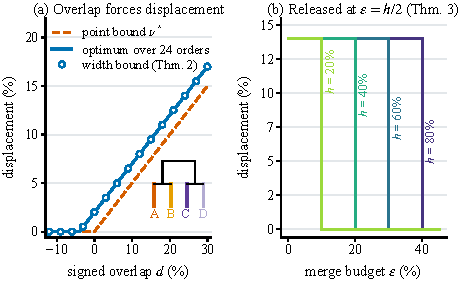
\includegraphics[width=\columnwidth]{figures/anchor_controlled_bounds.pdf}
\caption{Controlled four-leaf trees with the configuration of Fig.~\ref{fig:projection_conflict} (inset; references in Section~\ref{sec:bounds-eval}). (a) Increasing sibling-range overlap $d$ forces displacement; the width bound of Theorem~\ref{thm:width} (circles) equals the optimum over all 24 leaf orders. (b) At $d=24\%$, the 14\% displacement disappears exactly when the merge budget reaches half the parent gap $h$, for all four gaps, as Theorem~\ref{thm:chain} predicts. Percentages refer to a unit canvas or a unit scalar range.}
\label{fig:controlled}
\end{figure}
\begin{figure*}[t]
\centering
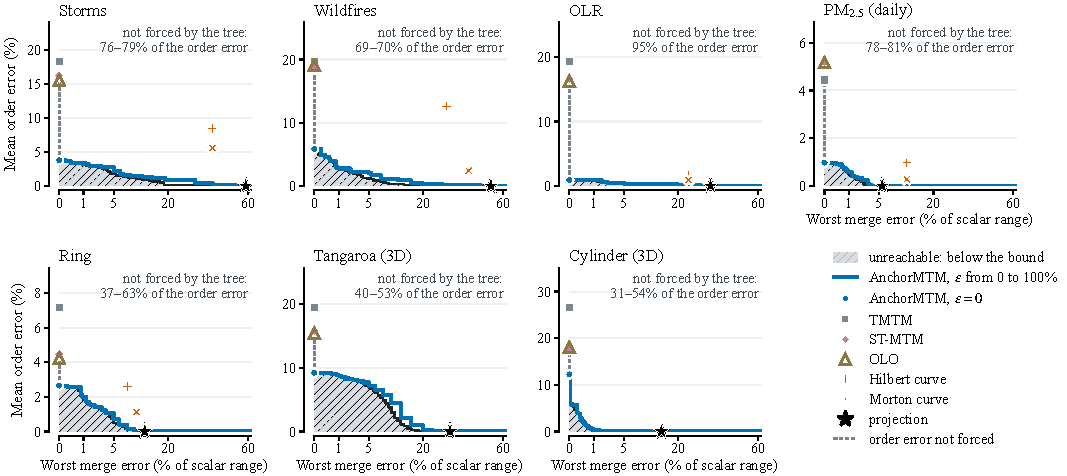
\includegraphics[width=\textwidth]{figures/plane_compact.pdf}
\caption{Position--topology plane of the bound suite, five planar and two volumetric sequences. Each map is one point: its worst merge error over frames (horizontal, square-root scale) and its mean order error (vertical). No map can enter the grey region below the bound (Theorem~\ref{thm:chain} and the flattened bound; Theorem~\ref{thm:order} at zero merge error). TMTM, ST-MTM and OLO keep the tree and sit at zero merge error far above the bound; on Storms, 76--79\% of their order error is not forced by the tree. Space-filling curves and the projection follow space and break the tree. AnchorMTM (blue, $\varepsilon$ from 0 to 100\%) runs along the edge; on Storms, OLR, daily PM$_{2.5}$ and Ring, enumerating all leaf orders shows that it is the exact optimum at every tested budget except one Storms frame. TMTM, ST-MTM and OLO are shown in the mirror that agrees better with the reference. All marks lie at their measured values, so marks at zero merge error can coincide; the dot is AnchorMTM at $\varepsilon=0$, and the Storms bar splits the order error of the tree-keeping maps into $\nu^*$ (black) and the rest (grey).}
\label{fig:plane}
\end{figure*}
We evaluate the bounds and the maps on two groups of sequences (Section~\ref{sec:data}). We first test whether the bounds are tight (Section~\ref{sec:bounds-eval}) and then use them to measure how much of the positional error of existing maps the tree forces (Section~\ref{sec:eval-forced}). We next compare where the methods place features at the same topological guarantee (Section~\ref{sec:eval-placement}), examine what a merge budget changes frame by frame (Section~\ref{sec:eval-budget}), and close with a case study on air pollution (Section~\ref{sec:reading}).

\begin{figure*}[t]
\centering
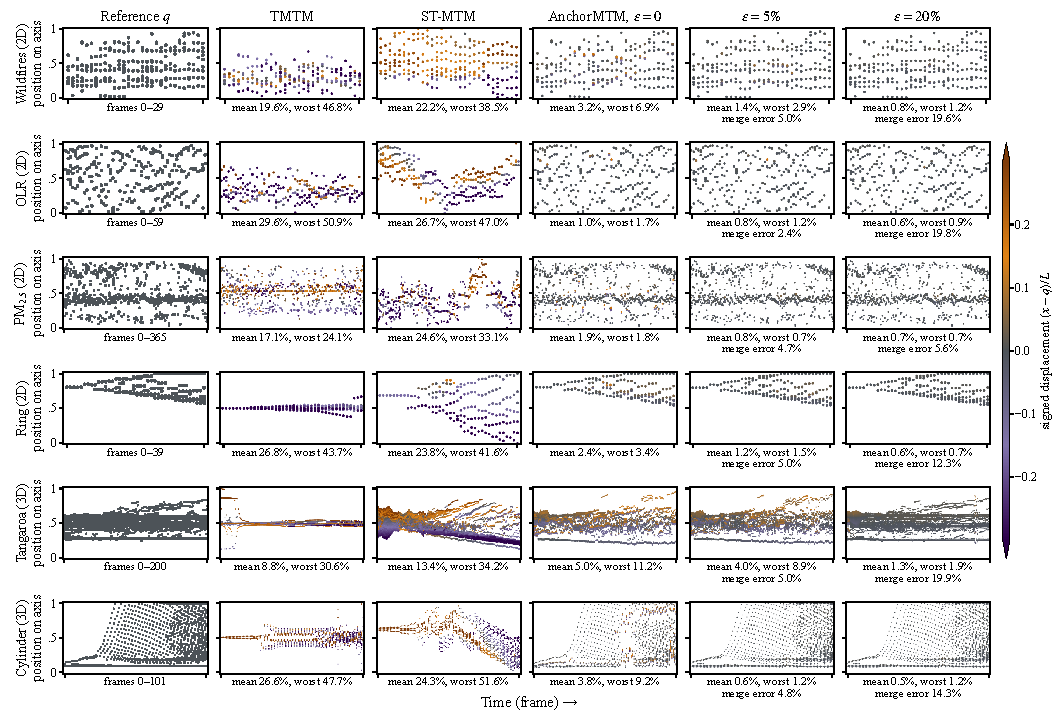
\includegraphics[width=\textwidth]{figures/volume_gallery.pdf}
\caption{Where each method draws the features of the two volumes. Each dot is one feature in one frame at its position on the axis (fraction of the canvas), colored by its signed displacement from its reference; grey dots lie on their references. The first column shows the references, that is, what a map read as location should show. All methods use the same trees and features; TMTM and ST-MTM are implementations of the published methods, each in the mirror that agrees better with the reference. AnchorMTM uses the default configuration of the bound suite with the matched-motion direction (Tangaroa) or the streamwise $x$ axis (Cylinder). Below each panel: mean and mean worst displacement over frames and, for a positive budget, the attained merge error.}
\label{fig:volume-gallery}
\end{figure*}
\subsection{Data and Protocol}\label{sec:data}
\begin{table}[t]
\centering
\caption{Two groups of sequences. The bound suite has saved trees and serves the bounds; the layout suite recomputes the trees and serves the comparison of complete maps.}
\label{tab:data}
\footnotesize
\setlength{\tabcolsep}{2pt}
\renewcommand{\arraystretch}{0.95}
\begin{tabular*}{\columnwidth}{@{\extracolsep{\fill}}lllr@{}}
\toprule
Suite & Sequence & Field & Frames \\
\midrule
Bound & Storms~\cite{Hersbach:2020:ERA5} & ERA5 sea-level pressure (12\,h) & 118 \\
 & Wildfires~\cite{Franke:2021:1DP} & fire radiative power, daily & 30 \\
 & OLR~\cite{NOAA:OLR} & outgoing longwave radiation & 60 \\
 & PM$_{2.5}$~\cite{Dong:2026:PM25} & PM$_{2.5}$ concentration, daily & 366 \\
 & Ring & synthetic ring & 40 \\
 & Tangaroa~\cite{Popinet:2004:Tangaroa} & velocity magnitude (3D) & 201 \\
 & Cylinder~\cite{Camarri:2005:Cylinder} & $Q$-criterion (3D) & 102 \\
\midrule
Layout & Gaussian & three moving peaks & 64 \\
 & Ring & synthetic ring & 40 \\
 & Wildfires & fire radiative power (32 bins) & 32 \\
 & Storms & ERA5 pressure anomaly (1\,h) & 744 \\
 & PM$_{2.5}$~\cite{Kong:2021:CAQRA} & PM$_{2.5}$ concentration, hourly & 744 \\
 & Tangaroa & velocity magnitude (3D) & 201 \\
 & Cylinder & $Q$-criterion (3D) & 102 \\
\bottomrule
\end{tabular*}
\end{table}

Table~\ref{tab:data} lists two groups of sequences. The \emph{bound suite} comes with the saved trees of an earlier benchmark, prepared with one extractor, matching rule and reference estimator and with one default configuration; on it we evaluate the bounds, all leaf orders of small frames and every compared map frame by frame (Sections~\ref{sec:bounds-eval} and~\ref{sec:eval-forced}). The \emph{layout suite} reconstructs the four planar inputs of the ST-MTM benchmark~\cite{STMTM:2026}, so that AnchorMTM is compared on the data of the closest prior work, and adds an hourly PM$_{2.5}$ sequence outside that benchmark and the two TMTM volumes~\cite{Koepp:2023:TMTM,Weinkauf:SquareCylinder} (Sections~\ref{sec:eval-placement} and~\ref{sec:eval-budget}). The hourly PM$_{2.5}$ sequence covers January 2017 over northern China (110--120$^\circ$E, 32--41$^\circ$N) with 744 reanalysis fields~\cite{Kong:2021:CAQRA} interpolated to $160\times144$; maxima are extracted as join trees of the negated field, with persistence 5\% of each frame's range. Ring, Storms, Wildfires and the volumes occur in both suites with different preprocessing (Supplementary Material), and the two PM$_{2.5}$ sequences are different data, daily in the bound suite and hourly in the layout suite. Author-processed arrays are unavailable, so the layout suite is a disclosed reconstruction, with the ST-MTM persistence numbers read as per-frame range fractions (0.1, 0.1, 15 and 10.5\%), not an identical-input reproduction.

\paragraph{Measures.} NMLE is the attained merge error $\dtop$ (Eq.~\ref{eq:dtop}) of the rendered profile divided by the scalar range, and NROE is the order error of Eq.~\ref{eq:nroe}. NPE is the worst displacement $\max_i|x_i^t-q_i^t|$ of a frame divided by the physical extent and averaged over frames. SNS is the scale-normalized stress between support-centroid and anchor distances~\cite{Smelser:2025:Scale,STMTM:2026}, and TW measures neighborhoods~\cite{Venna:2001:NP} with $k=(1,3,5,3)$, using only frames with $0<k<n_t/2$ (64/64, 1/40, 4/32 and 11/744), and with $k=1$ on all 744 PM$_{2.5}$ frames. On the four benchmark inputs, the SNS and TW of TMTM and ST-MTM in Table~\ref{tab:quantitative-final} are quoted from ST-MTM (Temporal mode, authors' inputs) and are not ranked against local values. All other baseline values are measured on our implementations of the published methods with the same trees, identities and references, with the Storms parameters of ST-MTM on PM$_{2.5}$. Each baseline map in Table~\ref{tab:quantitative-final} is reflected once for the whole sequence if its anchors and references correlate negatively on the first frame where both vary; Figs.~\ref{fig:plane} and~\ref{fig:volume-gallery} use the global mirror that agrees better with the reference. Hilbert and Morton curves keep a fixed grid orientation~\cite{Franke:2021:1DP}. The volumetric table uses the $+x$ axis chosen by an offline displacement rule and stored, tuned configurations (Supplementary Table~S4), whereas Figs.~\ref{fig:volume-gallery} and~\ref{fig:budget-distribution} use the default configuration of the bound suite.

\paragraph{Modes.} Exact is Exact Mode ($\varepsilon=0$). Balanced is Budgeted Mode with a positive budget selected from 1--10\% on the first chronological quarter by $J=0.5\,\mathrm{NPE}_{norm}+0.5\,\mathrm{SNS}_{norm}$ over candidates within their budget, preferring smaller budgets within 0.01 of the minimum, and frozen before the full runs at 1, 1, 5 and 10\% (Supplementary Fig.~S4). Earlier outputs had been observed, so this is not a blind test. PM$_{2.5}$ was added later with a fixed $\varepsilon=5\%$ that this rule did not select, and it is reported under its budget rather than as Balanced.

\paragraph{Implementation.} One cold Balanced run takes 0.5--63\,s on an Apple M4, of which ordering and placement take 0.15--3.3\,s; the remainder is preprocessing, tree extraction, matching, rasterization and checks. The 744-frame PM$_{2.5}$ run at 5\% takes 231\,s, 200\,s of it in ordering and placement. Supplementary Tables~S3 and~S4 list all settings, and Supplementary Fig.~S8 shows a joint guidance--topology sweep on Ring with source snapshots.

\begin{figure*}[t]
\centering
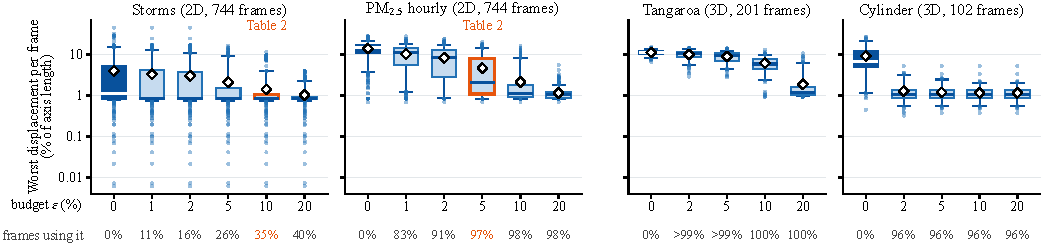
\includegraphics[width=\textwidth]{figures/budget_per_frame.pdf}
\caption{Per-frame worst displacement of AnchorMTM over the merge budget $\varepsilon$ on complete sequences (log scale): two planar inputs with the configuration of Table~\ref{tab:quantitative-final} and the two volumes with the default configuration. Boxes: quartiles; whiskers: 5th--95th percentiles; dots: all frames outside the whiskers, at their values; diamonds: means, the NPE of the tables; dark: Exact; orange: the budget of Table~\ref{tab:quantitative-final}. The bottom row gives the share of frames whose attained merge error is positive; no frame exceeds its budget. On Storms a budget shortens the upper tail; on PM$_{2.5}$ and in the volumes, almost every frame uses it and the whole distribution moves. Wildfires, Ring and per-frame merge errors: Supplementary Figs.~S1--S3.}
\label{fig:budget-distribution}
\end{figure*}
\subsection{Tightness of the Bounds}\label{sec:bounds-eval}
\emph{Controlled trees.} We fix two sibling pairs $\{A,B\}$ and $\{C,D\}$ that merge at $0.4$ below a root at $1$, with leaf values $0$ and references $(0.2,0.5,0.5-d,0.8-d)$ on a unit canvas; for $0<d<0.3$ this is the order $A,C,B,D$ of Fig.~\ref{fig:projection_conflict}. We vary the signed overlap $d$ from $-0.12$ to $0.30$ and, across 43 overlaps and four widths, compare the bounds with all 24 leaf orders, each placed by an independent minimax LP. Topology alone forces exactly $\nu^*=\max(0,d)/2$. With widths $0.06$, gap $0.01$ and $\rho=0.5$, the width bound, our search and the exhaustive optimum coincide at $\tau=\max(0,(d+0.04)/2)$ (Fig.~\ref{fig:controlled}a): 12\% for points and 14\% for intervals at $d=0.24$. A merge budget removes the conflict exactly where Theorem~\ref{thm:chain} admits interleaving, at $2\varepsilon=h$ for all four parent gaps $h$ (Fig.~\ref{fig:controlled}b).

\emph{Real trees.} In Exact Mode, the interval cost $\tau$ of the selected order equals $\mathcal{B}_w$ on 606 of the 614 planar frames of the bound suite, so on these frames no exact-topology order has a smaller worst displacement; at $\varepsilon=10\%$, the bounded-topology bound is met on 596. On Storms, OLR, daily PM$_{2.5}$ and Ring, every frame has at most eight leaves, and enumerating all leaf orders shows that the AnchorMTM order reaches the least order error at every tested budget, except one Storms frame at $\varepsilon=31.6\%$ (1.9 points). Volumes are harder: the width bound is met on 81 of 102 Cylinder and 27 of 201 Tangaroa frames, and the remaining gap may lie in the bound or in the heuristic search.

\subsection{Forced and Chosen Error of Existing Maps}\label{sec:eval-forced}
Theorem~\ref{thm:order} needs no layout, so it measures every exact-topology map, and midpoint ordering attains $\nu^*$ on the same tree. On the seven bound sequences, 53--95\% of the order error of TMTM and 31--95\% of that of ST-MTM lies above $\nu^*$ and is therefore chosen by their order rules (Supplementary Table~S2); OLO, which only optimizes adjacency within the tree, behaves alike (32--95\%). Figure~\ref{fig:plane} places every map in the position--topology plane. Maps that keep the tree sit at zero merge error far above the bound. The projection reaches zero order error only with merge errors of 5.6--59\%, and the space-filling curves also break the tree (8--40\%). AnchorMTM runs along the edge between them, and this edge shows what a budget releases. Where conflicting subtrees merge just below their parent, 1\% halves the forced order error on Wildfires (5.80\% to 2.77\%) and almost removes it on Cylinder (12.24\% to 0.23\%), whereas the deep conflicts of Tangaroa keep it above 7\% up to $\varepsilon=5\%$. The forced cost also depends on the direction and can be computed before any map is drawn: over 400 directions, it spans 4.70--10.14\% on Tangaroa and 5.49--28.15\% on Cylinder (Supplementary Fig.~S6).

\subsection{Placement at the Same Topological Guarantee}\label{sec:eval-placement}
\begin{table}[t]
\centering
\caption{Volumetric comparison with a fixed $x$ reference. Bold/underline mark best/second distinct values per dataset; ties share emphasis.}
\label{tab:volume-comparison}
\footnotesize
\setlength{\tabcolsep}{1.2pt}
\renewcommand{\arraystretch}{0.9}
\begin{tabular*}{\columnwidth}{@{\extracolsep{\fill}}lccc lccc@{}}
\toprule
\multirow{2}{*}{Dataset} & \multicolumn{3}{c}{TMTM} & \multicolumn{4}{c}{AnchorMTM (ours)} \\
\cmidrule(lr){2-4}\cmidrule(lr){5-8}
 & SNS$\downarrow$ & TW$\uparrow$ & NPE$\downarrow$ & Mode & SNS$\downarrow$ & TW$\uparrow$ & NPE$\downarrow$ \\
\midrule
\multirow{2}{*}{Cylinder} & \multirow{2}{*}{$0.2956$} & \multirow{2}{*}{$\underline{0.8017}$} & \multirow{2}{*}{$0.4769$} & Exact & $\underline{0.1226}$ & $0.8010$ & $\underline{0.1773}$ \\
 &  &  &  & Balanced & $\mathbf{0.0329}$ & $\mathbf{0.9117}$ & $\mathbf{0.0458}$ \\
\multirow{2}{*}{Tangaroa} & \multirow{2}{*}{$0.5255$} & \multirow{2}{*}{$0.6701$} & \multirow{2}{*}{$0.3866$} & Exact & $\underline{0.1204}$ & $\underline{0.8213}$ & $\underline{0.1285}$ \\
 &  &  &  & Balanced & $\mathbf{0.1124}$ & $\mathbf{0.8408}$ & $\mathbf{0.0653}$ \\
\bottomrule
\end{tabular*}
\vspace{2pt}
\begin{minipage}{\columnwidth}\footnotesize All values are local measurements, including adapted TMTM. TW uses $k=1$, with coverage 102/102 and 201/201. Mode applies only to AnchorMTM. Configurations are frozen exploratory results, not a blind test; settings appear in the supplement.\end{minipage}
\end{table}

\emph{Planar inputs.} At the same zero merge error, Exact lowers NPE relative to TMTM and ST-MTM by 73--96\% on all five inputs of Table~\ref{tab:quantitative-final} (73.5 and 75.1\% on PM$_{2.5}$), and it is also below the Hilbert and Morton curves, which break the tree. Balanced, with a budget of at most 10\%, lowers NPE relative to Exact by a further 16.2\% on Ring, 11.6\% on Wildfires and 64.9\% on Storms; Gaussian is unchanged, and the fixed 5\% budget lowers it by 66.3\% on PM$_{2.5}$. These results support alignment to a chosen reference, not a general gain in quality. ST-MTM reports a higher TW on all four benchmark inputs, and we do not rank its published SNS and TW, which come from the authors' inputs and coverage, against local values. On PM$_{2.5}$, where every score is local, ST-MTM also keeps a lower SNS and a higher TW than Exact (0.1897 and 0.8224 versus 0.1964 and 0.7884). Against the curves, Balanced improves SNS and TW on Gaussian, Wildfires and Storms, but Hilbert is better on Ring (SNS 0.1252 and TW 0.9048 versus 0.1334 and 0.8571, with TW from one eligible frame), Balanced raises SNS on Wildfires from 0.0426 to 0.0447, and both curves keep a higher TW than the 5\% map on PM$_{2.5}$.

\emph{One storm.} Figure~\ref{fig:storms_overview} shows what these averages mean for a single feature. As the storm moves from the Atlantic to Scandinavia, its reference rises from 0.08 to 0.86 of the axis. TMTM aligns subtrees by temporal overlap and ST-MTM places them by relative distance, so both keep the storm's band near the middle of the axis, and the band conveys neither the location of the storm nor the direction of its motion. With exact topology, AnchorMTM draws the storm on average 1.5\% of the axis from its reference, and a 10\% budget lowers this to 1.0\%. These maps use an hourly Storms archive prepared separately from Table~\ref{tab:quantitative-final}. The baselines are local implementations run on the same 744 fields and augmented trees; genuine multiway saddles are handled by equal-level separators (TMTM) or by an equal-level binary refinement whose leaf merge matrices are checked (ST-MTM).

\emph{Reading motion.} A spatial axis should also show whether two features approach or separate. On the four planar bound sequences with such events (Storms, Wildfires, OLR and Ring; 56--124 events in which the distance between two tracked features changes by more than 2\% of the domain diagonal within two frames), an anchored exact-topology layout misreads 5--32\% of the events, TMTM 39--65\% and ST-MTM 21--41\%, and neither baseline misreads fewer events on any sequence. The task involves relative distances, which ST-MTM fits directly, and it relates to the motion term of our placement, so it supports reading motion rather than providing independent evidence.

\emph{Volumes.} With the tuned configurations and the $+x$ reference of Table~\ref{tab:volume-comparison}, Exact lowers NPE at zero merge error from 0.477 to 0.177 on Cylinder and from 0.387 to 0.129 on Tangaroa, and Balanced improves all three metrics over TMTM; Tangaroa's 33.33\% budget and geometry-dominated weights limit attribution. Figure~\ref{fig:volume-gallery} shows the positions behind these numbers under the default configuration. TMTM and ST-MTM gather the Cylinder vortices near the middle of the axis (mean worst displacement 47.7\% and 51.6\%), whereas Exact already reproduces the shedding pattern of the references (9.2\%), and a 5\% budget removes almost all of the rest (1.2\%). The conflicts in Tangaroa are deep: Exact lowers 30.6\% (TMTM) and 34.2\% (ST-MTM) to 11.2\%, and the pattern of the references appears only near $\varepsilon=20\%$ (1.9\%).

\emph{Budgets.} Exact has zero measured merge error on every input. Balanced attains at most 0, 0.982, 4.421 and 9.985\%, within its budgets, and all runs pass the continuous and raster checks without collapsed anchors; Ring needs checked joint integer rounding in 26 Exact and 21 Balanced frames. In the volumetric sweeps, all 1,515 rendered frames were rechecked against the fixed-leaf merge matrices without a violation. The checks cover diagonal extrema, not every augmented internal label.

\subsection{Effect of the Merge Budget per Frame}\label{sec:eval-budget}
Figure~\ref{fig:budget-distribution} shows the budget frame by frame. Its effect depends on how many frames contain a conflict that it can release. On Storms, 35\% of the frames use the allowance at $\varepsilon=10\%$, in a few runs of consecutive frames (Supplementary Fig.~S2), so the budget shortens the upper tail: the median per-frame displacement moves only from 1.10\% to 0.84\%, while the 90th percentile falls from 10.7\% to 2.5\% and the worst frame from 44.8\% to 11.5\%. On Wildfires, the same 7 of 32 frames use the allowance at every budget, and on Ring the median falls from 3.9\% to 1.0\% while the last frame stays at 10.0\% until the budget reaches 63\% (Supplementary Fig.~S1). On hourly PM$_{2.5}$, 97\% of the frames use the 5\% budget, and the whole distribution moves: the median falls from 14.5\% to 2.1\%. The volumes behave alike. At a 2\% budget, 200 of 201 Tangaroa and 98 of 102 Cylinder frames use it; the Cylinder median falls from 6.8\% to 1.0\% already at 2\%, and the Tangaroa median from 11.3\% to 1.2\% at 20\%. A budget limits merge error, not displacement, so a positive budget need not change the map, as on Gaussian.

\subsection{Case Study: An Air-Pollution Episode}\label{sec:reading}
\begin{figure}[t]
\centering
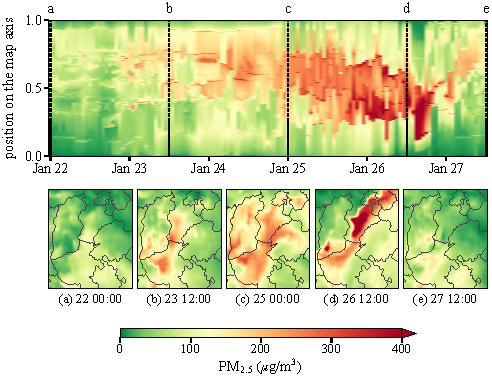
\includegraphics[width=\columnwidth]{figures/pm25_hourly.pdf}
\caption{An air-pollution episode in the hourly PM$_{2.5}$ sequence, 22--27 January 2017 (Beijing time), drawn by AnchorMTM with $\varepsilon=5\%$. Top: 133 hourly columns; dashed lines a--e mark the times of the snapshots below. Bottom: source fields over northern China. Concentrations above 400\,$\mu$g/m$^3$ saturate.}
\label{fig:pm25-hourly}
\end{figure}
Figure~\ref{fig:pm25-hourly} shows how an analyst can read an episode from the map alone and confirm it in the source fields. On 22 January the air is clean (a). On 23 January, orange bands appear in the upper half of the map, and the source field shows separate pollution maxima (b). By 25 January the polluted area covers much of the region, and the bands widen (c). The episode peaks on 26 January: the highest concentrations lie in a narrow belt (d), and the darkest bands descend on the map, that is, the strongest maxima move toward lower reference positions. By 27 January the air has largely cleared (e). Because the axis is anchored, a band that keeps its height is a maximum that stays at the same position along the reference direction while its concentration changes, whereas a band that drifts is a maximum that moves along this direction; on a map whose axis has no spatial meaning, the two cannot be told apart. The merge error stays within the budget in all 744 frames (at most 4.998\%).

\section{Discussion and Limitations}
\paragraph{Using the bounds.} The bounds split the error of any map into a part that the tree forces and a part that its layout chooses. Order error above $\nu^*$ can always be removed without changing the tree, because midpoint ordering attains $\nu^*$. The width-aware and bounded-topology bounds need not be attained, so an excess above them may lie partly in the bound. Because the bounds need only the tree, the projected locations and the widths, they can be computed before a map is drawn, to choose a direction or to decide whether a budget is worth spending, and any new layout of this family can be measured against them.

\paragraph{Position and neighborhoods.} A fixed spatial reference and a geometry-oriented embedding answer different questions. AnchorMTM supports reading positions and motion along a chosen direction; the higher TW reported by ST-MTM shows the value of preserving local neighborhoods, and neither property guarantees the other. Our results support this task-specific claim, not a general superiority in spatial or temporal fidelity. One axis also carries only one coordinate: reading two-dimensional positions would require a second map along another direction, with its own bound.

\paragraph{Limitations.} Author-processed fields and their small-sample TW protocol are not fully available, so the published SNS and TW cannot support an identical-input significance test, and the two suites differ in preprocessing. The reference and the tracks are computed offline from the whole sequence, and support overlap is a proxy for correspondence, not a physical identity. The order search is heuristic, and a continuous certificate does not remove raster rounding; we therefore check the rendered merge matrices, but not every augmented internal label. Reading motion assumes known identities. We have not measured perceptual readability, the accuracy of human motion judgments or generalization to unseen data; these require user studies.

\section{Conclusion}
Anchoring the axis of a merge tree map to space has an unavoidable positional price. By writing merge tree maps as one layout problem, with TMTM and ST-MTM as exact-topology instances, we bound this price for every instance. The bounds are attained on 606 of 614 planar benchmark frames, and 31--95\% of the order error of TMTM and ST-MTM is not forced by the tree. AnchorMTM pays little more than the price: at the same zero merge error, it lowers the mean worst displacement by 73--96\% on the four ST-MTM benchmark inputs and hourly PM$_{2.5}$, and a declared merge budget, verified on every rendered frame, buys further position where conflicts are shallow. ST-MTM's published neighborhood preservation remains higher, which marks the trade-off between reading locations and reading neighborhoods.
% Flush pending floats without forcing an otherwise empty bibliography page.
\FloatBarrier
\begingroup
\interlinepenalty=10000
\bibliographystyle{abbrv-doi-narrow}
\bibliography{refs}
\endgroup
\end{document}
